
\section{Friday}\index{week7_Thursday_lecture}
\paragraph{Announcement}
Our final exam is on $2018.12.16$ (Sunday), one day before the final exam. The exact time depends on the room schedule. Today we are going to talk about the improper integral, which is the last topic in the chapter Riemann integration.

\subsection{Improper Intergrals}
\paragraph{Motivation}
So far, to define the integration, we pre-assume $f$ and the interval are bounded. In practice, however, we are faced two situations:
\begin{enumerate}
\item
Interval may be unbounded, i.e., $(-\infty,b],[a,\infty),(-\infty,+\infty)$.

For example, how to define the integration of $f$ over $[a,\infty)$? A reasonable definition is
\[
\int_a^\infty f(x)\diff x:=\lim_{b\to\infty}\int_a^bf(x)\diff x
\]
\item
$f$ is unbounded. Specially speaking, $f$ may be defined on $[a,b)$ with limit to $b$ as infinity.

In such a situation, similarly, a reasonable definition is
\[
\int_a^bf(x)\diff x=\lim_{\varepsilon\to0+}\int_a^{b-\varepsilon}f(x)\diff x
\]
\end{enumerate}
\begin{example}
\begin{enumerate}
\item
Given the integral 
\begin{align*}
\int_0^1\frac{1}{x^{\alpha}}\diff x&=\lim_{\varepsilon\to0+}\int_\varepsilon^1\frac{1}{x^{\alpha}}\\
&=
\left\{
\begin{aligned}
\lim_{\varepsilon\to0+}\left[\frac{1}{(1-\alpha)x^{\alpha-1}}|_{\varepsilon}^1\right],\qquad \alpha\ne1\\
\lim_{\varepsilon\to0+}\left[\ln x|_{\varepsilon}^1\right],\qquad \alpha=1\\
\end{aligned}
\right.\\
&=
\left\{
\begin{aligned}
\frac{1}{1-\alpha},\quad \alpha<1\\
\infty,\qquad \alpha\ge1\\
\end{aligned}
\right.\\
\end{align*}
We have a function that is unbounded on $[0,1]$ but may have a bounded region (integration) over this interval. The interpretation is that whether the integration of $\frac{1}{x^{\alpha}}$ is bounded depends on the increasing rate of this function. (not \emph{singular} too much)
\item
Another example:
\begin{align*}
\int_1^\infty\frac{1}{x^{\alpha}}\diff x&=\lim_{b\to\infty}\int_1^b\frac{1}{x^{\alpha}}\\
&=
\left\{
\begin{aligned}
\lim_{b\to\infty}\left[\frac{1}{(1-\alpha)x^{\alpha-1}}|_{1}^b\right],\qquad \alpha\ne1\\
\lim_{b\to\infty}\left[\ln x|_{1}^b\right],\qquad \alpha=1\\
\end{aligned}
\right.\\
&=
\left\{
\begin{aligned}
\frac{1}{1-\alpha},\quad \alpha>1\\
\infty,\qquad \alpha\le1\\
\end{aligned}
\right.\\
\end{align*}
The interpretation, in this case, whether the integration of $\frac{1}{x^{\alpha}}$ is bounded depends on the decreasing rate of this function. (decreasing/converging fast enough)
\end{enumerate}
\end{example}
We summary the examples above as a useful proposition:
\begin{proposition}[Convergence of Reciprocal Integration]\quad
\begin{enumerate}
\item
The integral $\displaystyle\int_0^1\frac{1}{x^{\alpha}}\diff x$ with $\alpha>0$,
\begin{itemize}
\item
Converges if $\alpha<1$;
\item
Diverges if $\alpha\ge1$
\end{itemize}
\item
The integral $\displaystyle\int_1^\infty\frac{1}{x^{\alpha}}\diff x$ with $\alpha>0$,
\begin{itemize}
\item
Converges if $\alpha>1$;
\item
Diverges if $\alpha\le1$
\end{itemize}
\end{enumerate}
\end{proposition}





\paragraph{Notations}
We define the general integrals as $\int_a^wf$, where $w$ can be finite, i.e., normal integrals; or $w=\infty$, i.e., improper integrals.
\begin{definition}
The improper integral $\int_a^wf$ is said to be
\begin{enumerate}
\item
\emph{Absolute convergent}, if $\int_a^w|f|$ converges;
\item
\emph{Conditionally convergent}, if $\int_a^wf$ converges while $\int_a^w|f|$ diverges.
\end{enumerate} 
\end{definition}
\begin{proposition}[Comparison Test]
If $0\le f(x)\le g(x)$ on $[a,w)$, then 
\begin{enumerate}
\item
$\int_a^wg$ converges implies that $\int_a^wf$ converges; 
\item
$\int_a^wg$ diverges implies that $\int_a^wf$ diverges; 
\end{enumerate}
\begin{remark}
When determining the convergence of improper integral $\int_a^wf\diff x$ using comparison test, we usually compares it with the reciprocal integral $\int_a^w\frac{1}{x^\alpha}\diff x$, with the parameter $\alpha$ appropriately chosen.
\end{remark}
\end{proposition}
\begin{proposition}[Integral $\&$ Series Test]\label{Pro:7:4}
Let $f:[1,\infty)\mapsto\mathbb{R}$ be a non-negative, non-increasing, integrable function on every closed interval $[1,b]\subseteq[1,\infty)$. Then the series $\sum_{n=1}^\infty f(n)$ and the integral $\int_1^\infty f(x)\diff x$ either both converge or both diverge.
\end{proposition}
\begin{figure}[H]
\centering
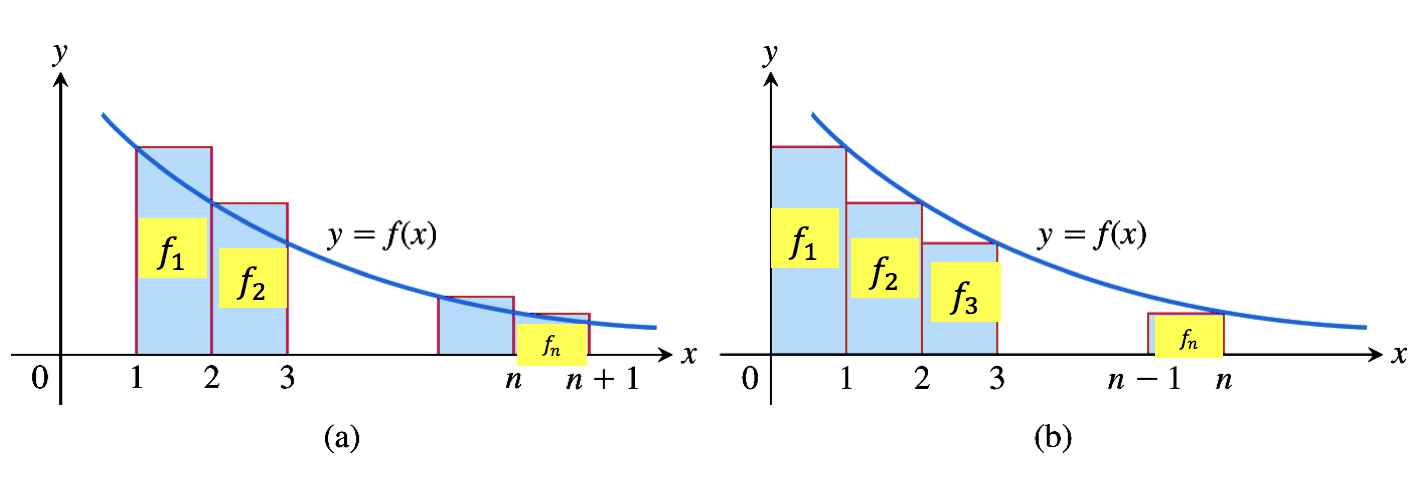
\includegraphics[width=15cm]{week7/f_1}
\caption{Graphic Interpretation of Proposition(\ref{Pro:7:4})}
\label{Geo_7_1}
\end{figure}
\paragraph{Graphic Interpretation of Proposition(\ref{Pro:7:4})}
Clearly, from Fig.(\ref{Geo_7_1}a), we derive
\begin{equation}\label{Eq:7:10}
\int_1^\infty f(x)\diff x\le f(1)+f(2)+\cdots+f(n)+\cdots
\end{equation}
Conversely, from Fig.(\ref{Geo_7_1}b), we derive
\begin{equation}\label{Eq:7:11}
f(2)+f(3)+\cdots+f(n)+\cdots\le\int_1^\infty f(x)\diff x
\end{equation}
\begin{proof}[A rigorous proof]
Let's reformulate (\ref{Eq:7:10}) and (\ref{Eq:7:11}) a little bit to make it more rigorous:
\begin{subequations}
\begin{align}
\sum_{k=1}^nf(k)&\ge\sum_{k=1}^n\int_k^{k+1}f(x)\diff x=\int_1^{n+1}f(x)\diff x\label{Eq:7:12:a}\\
\sum_{k=2}^nf(k)&\le \sum_{k=2}^n\int_{k-1}^{k}f(x)\diff x
=
\int_1^nf(x)\diff x\label{Eq:7:12:b}
\end{align}
\end{subequations}
\begin{itemize}
\item
From (\ref{Eq:7:12:a}), if $\int_1^\infty f(x)$ diverges, i.e., $\lim_{n\to\infty}\int_1^{n+1}f(x)\diff x=\infty$, then the sequence of partial sums heads off to infinity as well, i.e., the series diverges. The contrapositive is also true, i.e., the series converges implies that the integral converges.
\item
From (\ref{Eq:7:12:b}), if $\int_1^\infty f(x)$ converges, which bounds the sequene of partial sums, we imply that the series converges. The contrapositive is also true, i.e., if the series diverges, so does the integral.
\end{itemize}
\end{proof}

\begin{example}
Determine the convergence of the following integrals:
\begin{subequations}
\begin{enumerate}
\item
\begin{equation}\label{Eq:7:13:a}
\int_1^\infty\frac{\sqrt{x}}{\sqrt{1+x^4}}
\end{equation}
Note that $\frac{\sqrt{x}}{\sqrt{1+x^4}}\sim\frac{c}{x^{3/2}}$, and therefore (\ref{Eq:7:13:a}) converges
\item
\begin{equation}\label{Eq:7:13:b}
\int_1^\infty\exp(-x^2)\diff x
\end{equation}
Note that $\exp(-x^2)$ converges much faster than $x^{-\alpha},\alpha>1$, and thus (\ref{Eq:7:13:b}) converges.
\item
\begin{equation}
\int_2^\infty \ln x\diff x
\end{equation}
We can compute $\int_2^\infty \ln x\diff x$ directly:
\[
\int_2^\infty \ln x\diff x=[x\ln x-x]_{x=2}^{\infty}=\infty.
\]
\item
\begin{equation}(\label{Eq:7:13:d})
\int_0^{\pi/2}\ln(\sin x)\diff x
\end{equation}
Note that $\sin x\sim x\implies \ln(\sin x)\sim \ln x$. Also, $\ln x$ increases slower than $x^{-\alpha},\alpha<1$:
\[
\frac{\ln x}{\sqrt{x}}=\frac{1/x}{\frac{1}{2}\frac{1}{(\sqrt{x})^3}}=2x^{1/2}\to0,
\]
and therefore (\ref{Eq:7:13:d}) converges.
\item
\begin{equation}
\int_0^1\frac{\diff x}{\sqrt{(1-x^2)(1-k^2x^2)}},\quad 0\le k^2<1\qquad
\mbox{[Elliptic Integral]}\label{Eq:7:13:e}
\end{equation}
We reformulate it a little bit:
\[
\int_0^1\frac{\diff x}{\sqrt{(1-x^2)(1-k^2x^2)}}
=
\int_0^1\frac{\diff x}{\sqrt{(1+x)(1-k^2x^2)}}\frac{1}{\sqrt{1-x}}\sim\int_0^1\frac{\diff\eta}{\sqrt{\eta}},
\]
and therefore (\ref{Eq:7:13:e}) converges.
\item
\begin{equation}
\int_0^\phi\frac{\diff\theta}{\sqrt{\cos\theta-\cos\phi}},\quad 0<\phi<\frac{\pi}{2}\label{Eq:7:13:f}
\end{equation}
Note that
\[
\cos\theta-\cos\phi=-2\sin\frac{\theta+\phi}{2}\sin\frac{\theta-\phi}{2}\sim\phi-\theta\implies
\frac{1}{\sqrt{\cos\theta-\cos\phi}}\sim\frac{1}{\sqrt{x}},
\]
and therefore (\ref{Eq:7:13:f}) converges.
\item
\begin{equation}
\int_{\pi/2}^\infty\frac{\sin x}{x}\diff x
\label{Eq:7:13:g}
\end{equation}
We solve this problem via integration by parts:
\[
\int_{\pi/2}^b\frac{\sin x}{x}\diff x=-\frac{1}{b}\cos b-\int_{\pi/2}^b\frac{\cos x}{x^2}\diff x
\]
Note that $\int_{\pi/2}^b|\cos\frac{\cos x}{x^2}|\diff x\le\int_{\pi/2}^b\frac{1}{x^2}$, and thus this integral converges. However, this integral diverges, since the integration
\[
\int_{\pi/2}^\infty|\frac{\sin x}{x}|\diff x
\]
diverges. In summary, $\int_{\pi/2}^b\frac{\sin x}{x}\diff x$ is conditionally convergent.
\begin{proof}[proof for divergence of $\int_{\pi/2}^\infty|\frac{\sin x}{x}|\diff x$]
\begin{equation}\label{Eq:7:13:h}
\int_{\pi/2}^\infty|\frac{\sin x}{x}|\diff x\ge\int_{\pi/2}^\infty\frac{\sin^2 x}{x}\diff x=\int_{\pi/2}^\infty\frac{1}{2x}\diff x-\frac{1}{2}\int_{\pi/2}^\infty\frac{\cos 2x}{2x}\diff x,
\end{equation}
where the same trick shows that $\int_{\pi/2}^\infty\frac{\cos 2x}{2x}\diff x$ converges, and hence the subtraction (\ref{Eq:7:13:h}) diverges.
\end{proof}
\begin{proof}[Alternative proof for divergence of $\int_{\pi/2}^\infty|\frac{\sin x}{x}|\diff x$]
Consider the graph of $|\sin x|$:
\begin{figure}[H]
\centering
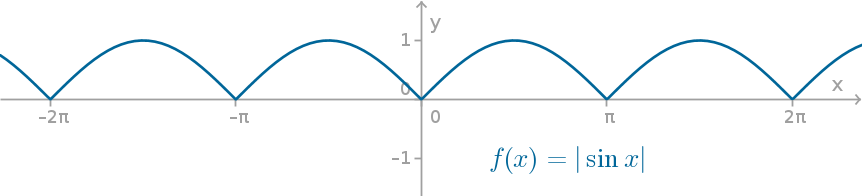
\includegraphics[width=10cm]{week7/f_2}
\caption{Graphic of $|\sin x|$}
\label{Geo_7_2}
\end{figure}
Thus the integrations of $|\sin x|$ over the interval $[2\pi n,(n+1)2\pi]$ are always the same:
\[
\int_{2\pi n}^{2\pi(n+1)}|\sin x|\diff x=\int_0^{2\pi}|\sin x|\diff x=4,\qquad n\in\mathbb{N}
\]
which follows that
\begin{align}
\int_0^{2\pi N}|\frac{\sin x}{x}|\diff x&=\sum_{n=0}^{N-1}\int_{2\pi n}^{2\pi(n+1)}|\frac{\sin x}{x}|\diff x\\
&\ge \sum_{n=0}^{N-1}\frac{1}{2\pi(n+1)}\int_{2\pi n}^{2\pi(n+1)}|\sin x|\diff x\label{Eq:7:13:l}\\
&=\sum_{n=0}^{N-1}\frac{1}{2\pi(n+1)}\int_{0}^{2\pi}|\sin x|\diff x\\
&=\sum_{n=0}^{N-1}\frac{2}{\pi(n+1)}\label{Eq:7:13:j}
\end{align}
where in (\ref{Eq:7:13:l}) we lower bound the $\frac{1}{|x|}$ as $\frac{1}{n+1}$ for each $n$. The last sum (\ref{Eq:7:13:j}) diverges as $N\to\infty$, and so does the original integral $\int_0^\infty |\frac{\sin x}{x}|\diff x$.
\end{proof}
\end{enumerate}
\end{subequations}
\end{example}














